\documentclass[english]{beamer}
\usepackage[utf8,latin9]{inputenc}
%%\usepackage[latin9]{inputenc}
\usepackage[T1]{fontenc}
\usepackage{babel}

\usepackage{beamerthemesplit}
\usetheme{Warsaw}
\beamertemplatetransparentcovered

\title{2 years of Londiste}
\author{Dimitri Fontaine}
\date{May, 21 2010}

\begin{document}

\frame{\titlepage}

\section*{Agenda}
\frame{
  \frametitle{Content}
  \tableofcontents[pausesections]
}

\section{Hi-Media Activities}
\frame{

 Online multimedia services: 

 \begin{itemize}
   \item Electronic payment

     \textit{8 millions of transactions, monthly, under constant growth}

   \item Advertising

     \textit{4 billions pages seen, monthly, up to 4000tps}

   \item Interactive Call Services

     \textit{4 millons calls, that's 200 000 hours, monthly}

  \end{itemize}
}

\section{Tool Set for production}

\subsection{Free Software \& Open Source Tools}
\frame{
  \frametitle{Open Source Tools}

  We're basically using only Open Source Software in production.

  \begin{itemize}
   \item Apache, haproxy, Nginx
   \item PHP, some tools are in python
   \item Linux, debian, FreeBSD
   \item PostgreSQL with \textit{contribs} and \textit{extensions}
  \end{itemize}
}

\frame{
  \frametitle{PostgreSQL and extensions}

  History makes it so that we're running a mix of \texttt{8.2}, \texttt{8.3}
  and \texttt{8.4}, with

  \begin{itemize}
   \item Skytools: PGQ, Londiste, walmgr, plproxy, pgbouncer
   \item \texttt{prefix\_range} datatype and indexing
   \item temporal, with the \texttt{period} datatype and indexing
   \item ip4r, accelerating \textit{GeoIP} matching
   \item pg\_freespacemap, for munin 
   \item UUID in 8.2
   \item orafce
  \end{itemize}
}

\frame{
  \frametitle{pgFouine} 

  \texttt{pgFouine} parses and analyses our logs 

\begin{itemize}
    \item<1-> it produces easy to digest \texttt{HTML} reports
    \item<2-> we script it for sending emails with the errors, too
    \item<3-> allows for targetting the optimisation effort
\end{itemize}

}

\subsection{Production Environment}
\frame{
  \frametitle{Production}

  Using from \texttt{8.2} to \texttt{8.4} in production:
	
  \begin{itemize}
    \item<1-> about 50 production databases
    \item<1-> anywhere from some \texttt{MB} to \texttt{1518 GB}
    \item<2-> OLTP (\textit{very low latency})
    \item<2-> OLAP (\textit{bigger volumes, high insert load})
    \item<3-> using distribution packages only
  \end{itemize}
}

\subsection{Human Resources}
\frame{
  \frametitle{I just work there}
  We're 2 DBA with a high specialisation on PostgreSQL. What we do is

  \begin{itemize}
    \item<1-> manage the production 
    \item<2-> participate into development (lots of logic is in the database)
    \item<3-> enhance the tool set, proposing and releasing Open Source
      Software each time it makes sense
  \end{itemize}
}

\subsection{Monitoring \& Performances}
\begin{frame}[fragile]
  \frametitle{Monitoring with munin \& nagios}
  \begin{overprint}
  \onslide<1>
  \begin{center} 
    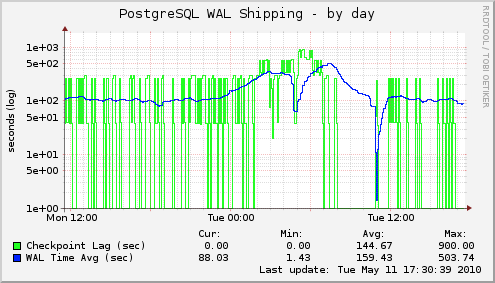
\includegraphics[height=2.4in]{bdd-pg_walmgr-day.png}
  \end{center} 

  \onslide<2>
  \begin{center} 
    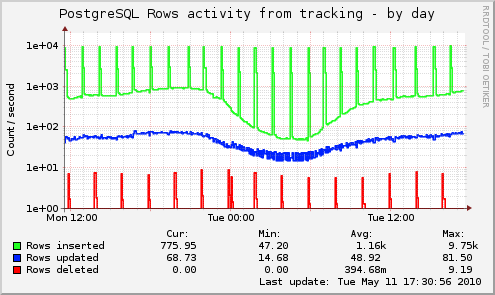
\includegraphics[height=2.4in]{tr1-pg_user_tables_activity_tracking-day.png}
  \end{center} 

  \onslide<3>
  \begin{center} 
    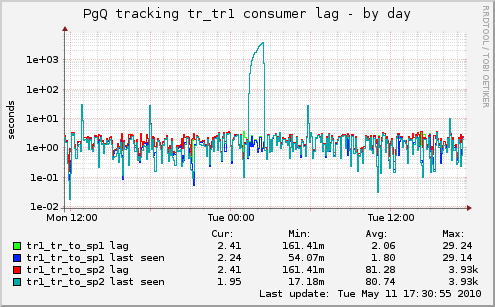
\includegraphics[height=2.4in]{tr1-pg_queue_tracking_tr_tr1-day.png}
  \end{center} 

  \onslide<4>
  \begin{center} 
    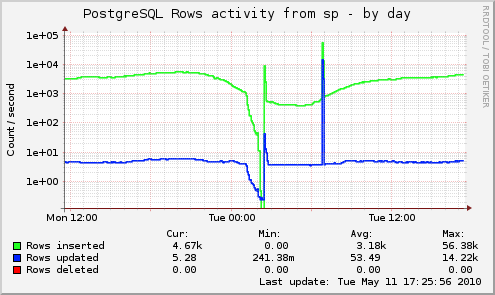
\includegraphics[height=2.4in]{sp2n-pg_user_tables_activity_sp-day.png}
  \end{center} 

  \end{overprint}  
\end{frame}

\frame{
  \frametitle{Good performance results}

  \begin{overprint}
    \onslide<1-4>

    Advertising

    \begin{itemize}
    \item<1-> About \texttt{6ms} to push an advert
    \item<1-> \texttt{300 tps} in average
    \item<2-> replication lag is setup for averaging at \texttt{3s}
    \item<3-> materialized views updated every 5 minutes
    \item<4-> switched from a mixed solution, so much better with only PostgreSQL
    \end{itemize}

    \onslide<5-7>

    Micro Payment

    \begin{itemize}
    \item<5-> Backoffice and reporting database, \texttt{190 GB}, running 8.4
    \item<5-> \texttt{64GB RAM}, \texttt{log\_min\_duration\_statement = 200ms}
    \item<6-> Slow queries are \texttt{COPY}, that's \textit{backups}
    \item<7-> Some other slow queries, slowest takes \texttt{0.51s} to run
    \end{itemize}

    \onslide<8-10>

    Telephony, IVR

    \begin{itemize}
    \item<8-> Answering phone calls, prefix lookups, running 8.3
    \item<8-> application status monitoring in the database, and replicated
    \item<9-> 500 updates a second, \texttt{HOT} + \texttt{CLUSTER}
    \item<10-> Statistics reports, backoffice, federating data, computing costs
    \end{itemize}
  \end{overprint}  
}

\section{Replication and failover}

\subsection{Different Architectures for different needs}

\frame{
  \frametitle{3 projects, 3 architectures, one tool set}

  We have 3 very different projects here, we're using specialised
  architectures but the same tools.

  \begin{center} 
    Let's see.
  \end{center} 
}

\frame{
  \frametitle{Centralised management and data federating}

  All server are both \textit{master} and \textit{slave}. Each IVR server is
  a master in its own schema.

  \begin{center} 
    \includegraphics[height=1.6in]{architecture_e}
  \end{center} 
}

\frame{
  \frametitle{Separating payments and their backoffice}

  The business critical part is the payment, it's running separated from the
  backoffice, but that's where customers will setup what they sell through
  our services.

  \begin{center} 
    \includegraphics[height=1.7in]{architecture_a}
  \end{center} 

}

\frame{
  \frametitle{Modernizing distributed delivery}

  A 3-stage processing of advert printing, from backoffice and setup to
  dynamic servers, with advert choice caped on budgets.

  \begin{center} 
    \includegraphics[height=2.1in]{architecture_c}
  \end{center} 
}

\subsection{A unique solution: Skytools}

\frame{
  \frametitle{Replication, Queuing}

  We use Skype tool suite, which is Open Source

  \begin{definition}
    \alert{\texttt{londiste}} Asynchronous master/slave replication

    \alert{\texttt{PGQ}} Queuing and asynchronous batches, still transactional

    \alert{\texttt{WalMgr}} WAL Shipping (\textit{failover})

    \alert{\texttt{pgbouncer}} connection pooling (\textit{prepared statements!})

    \alert{\texttt{plproxy}} alternative transport mechanism, and RPC solution
  \end{definition}
}

\frame{
  \frametitle{Maintenance: anecdotes from running Londiste}

  \begin{itemize}
  \item<1-> Had to replay 2 days of production: took 12 hours, 400 millions
    of events from 12 queues
  \item<1-> Got a hick-up of 15s when truncating the queue tables
  \item<2-> Other problems we had are all misbehavior of admins
  \item<2-> Typical is DDL on master only
  \end{itemize}
}

\frame{
  \frametitle{Using PGQ for batch needs}

  We have all this code in PHP, and we need to process data after the client
  saw the \texttt{COMMIT} back. We want to be able to stop them and never
  lose a single transaction, even if system crashes. PostgreSQL level
  reliability. \texttt{PGQ} offers that, for \texttt{python}.

  %% \linebreak
  %% \linebreak
  %% \pause

  \begin{center} 
    Enters \texttt{libphp-pgq} 
  \end{center}
}

\section{Conclusion}

\subsection{Reliable and flexible solution}

\frame{
  \frametitle{Multiple usages of replication}

  We use replication for serving quite different needs

  \begin{itemize}
    \item<1-> Separating different application layers
    \item<2-> Federating logs and offloading their processing
    \item<3-> Managing information on 1 backoffice only, but having network
      glitches tolerant front servers, or cached data if you will
    \item<4-> Materialized views for more than one server
    \item<5-> \textit{Failover} ready
  \end{itemize}
}

\frame{
  \frametitle{Reliability}

  We're experiencing very few hick-ups in production.
  \linebreak
  \linebreak

  From January 2009, I've been woken up less than 10 times for 4 projects
  and about 50 databases in production, and my colleague the same. On those
  night calls, a majority is application problems.
  \linebreak
  \linebreak

  It's not PostgreSQL disturbing my sleeping patterns (hi Kids)!
}

\subsection{Community}
\frame{
  \frametitle{What does it mean, this ``community''?}

  One of the main advantages of PostgreSQL is its community, delivering
  amazing extensions. From Skytools to temporal (period), we depend on the
  community about as much as from the core database engine.

  \pause
  \begin{center} 
    Being part of this community is as simple as picturing yourself as being
    part of it!
  \end{center}

  \pause
  \begin{center} 
    Welcome aboard!
  \end{center}
}

\subsection{Any question?}

\frame{
  \frametitle{Any question?}

  \begin{center}
    Now is a pretty good time to ask!
  \end{center}

  %% \linebreak
  %% \pause
  %% \begin{center}
  %%   If you want to leave feedback, consider visiting
  %%   \url{http://2009.pgday.eu/feedback}
  %% \end{center}
}


\end{document}


